% Created 2019-06-13 Thu 03:25
% Intended LaTeX compiler: pdflatex
\documentclass[11pt]{article}
\usepackage[utf8]{inputenc}
\usepackage[T1]{fontenc}
\usepackage{graphicx}
\usepackage{grffile}
\usepackage{longtable}
\usepackage{wrapfig}
\usepackage{rotating}
\usepackage[normalem]{ulem}
\usepackage{amsmath}
\usepackage{textcomp}
\usepackage{amssymb}
\usepackage{capt-of}
\usepackage{hyperref}
\usepackage{minted}
\author{Nicolás Luarte}
\date{\today}
\title{Johans}
\hypersetup{
 pdfauthor={Nicolás Luarte},
 pdftitle={Johans},
 pdfkeywords={},
 pdfsubject={},
 pdfcreator={Emacs 25.2.2 (Org mode 9.2.3)}, 
 pdflang={English}}
\begin{document}

\maketitle
\tableofcontents

\section{Ciclos}
\label{sec:org2fdca49}
\subsection{Ciclo 1:}
\label{sec:org060a5ab}
\begin{center}
\begin{tabular}{lll}
\hline
Ejercicio & Protocolo & Bloque\\
\hline
Press banca de competencia & x1@8, 20\%, 4x5 & A\\
Press banca pies arriba & x1@8, 20\%, 2x5 & A\\
Press banca con mancuernas & x10@7, 8, 9, 2x10 & A\\
Skull crushers con mancuernas & x10@7, 8, 9, 2x10 & A\\
\hline
Press banca de competencia tempo 600 & x1@8, 20\%, 4x4 & B\\
Press banca agarre cerrado & x10@8, 10\%, 2x10 & B\\
Remos con mancuerna & x10@7, 8, 9, 2x10 & B\\
Press militar con mancuerna & x10@7, 8, 9, 2x10 & B\\
\hline
\end{tabular}
\end{center}
\section{Comentarios técnicos}
\label{sec:org16ac155}
\subsection{11/06/2019 ciclo 1, bloque a:}
\label{sec:org86f3ba4}
\subsubsection{Press banca de competencia:}
\label{sec:org3072c8b}

\begin{enumerate}
\item Ajustar mejor el RPE, hubo ligero undershoot (un poquito mas bajo
de lo esperado)
\item La planta del pie debe estar completamente apoyada en el suelo
\item Para tomar la barra, rotar internamente las manos (un poco) de
manera tal que la barra descanse mas abajo en la palma
\item Aplicar "pausa activa", esto quiere decir, que la barra apenas toca
la primera fibra de tú polera, no debe hundirse en tú pecho.
\end{enumerate}

\subsubsection{Press banca pies arriba:}
\label{sec:orgbfb8a13}

\begin{enumerate}
\item Aplicar "pausa activa" y rotación de muñecas como especifique
arriba
\item Dejar los pies estirados
\item undershoot de RPE
\end{enumerate}

\subsubsection{Press banca con mancuernas:}
\label{sec:org4b5c401}

\begin{enumerate}
\item Undershoot de RPE
\end{enumerate}

\subsection{12/06/2019 ciclo 1, bloque b:}
\label{sec:orgf53f34b}
\subsubsection{Press banca de competencia tempo 600}
\label{sec:orgf2c0c55}
\begin{enumerate}
\item Seguir trabajando el tocar la fibra de la polera, ahora agregando
el gesto de llevar el pecho hacia la barra, de manera activa
\item Ligeramente ir aumentando la rotación de la muñeca al tomar la
barra
\item Al momento de subir estás haciendo mucho "flare" con los codos, es
decir, los codos se te abren mucho, hasta cierto punto eso es
deseable, pero en este caso fue mucho, busca que al salir del pecho
los codos no se muevan tanto y permanezcan en su posición
\end{enumerate}
\subsubsection{Press banca agarre cerrado}
\label{sec:orgad48579}
\begin{enumerate}
\item Dado que este es un movimiento poco técnico, no hay muchas
correcciones que hacer, solo orientarlo a una conexión
mente-musculo mientras lo realizas, para obtener la mayor cantidad
de beneficio posible de esta variante, que tiene como foco
principal la hipertrofia
\end{enumerate}

\section{Registro de progreso}
\label{sec:orga337e63}
\begin{center}
\label{tab:org3185ff3}
\begin{tabular}{lrrl}
Ejercicio & RPE & Peso & Fecha\\
\hline
Press banca de competencia & 7 & 92 & 11/06/2019\\
Press banca pies arriba & 7.5 & 85 & 11/06/2019\\
Press banca de competencia tempo 600 & 8 & 87.5 & 12/06/2019\\
Press banca agarre cerrado & 8 & 58 & 12/06/2019\\
\end{tabular}
\end{center}
\begin{center}
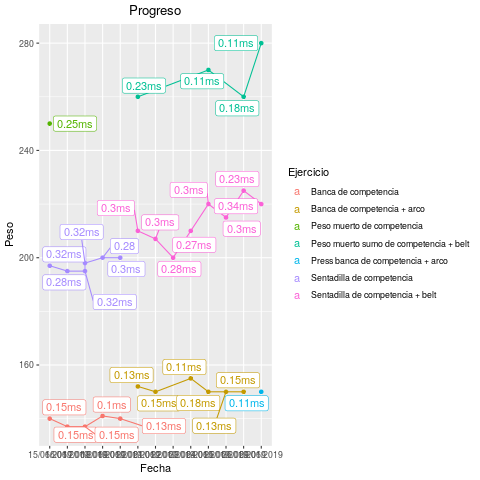
\includegraphics[width=.9\linewidth]{tmp.png}
\end{center}
\end{document}
